\documentclass{beamer}
\usepackage{etoolbox}\newtoggle{printable}\togglefalse{printable}
\usetheme{Copenhagen}
\usecolortheme{beaver}
\usepackage{listings}
\usepackage{algpseudocode}
\pdfmapfile{+sansmathaccent.map}
\graphicspath{ {Images/} }

\title{Comp240 Market Evaluation \& Business Case}
\author{Alastair Rayner}
\date{\today}

\begin{document}

\maketitle


% ////////////////// TARGET AUDIENCE
\begin{frame}{About the Product}
	The product I have been working on is a lobby system for the BA team Firelock. \pause
	
	This presentation will aim to address whether there is an audience for the game being developed by Firelock, and furthermore which marketing strategy we believe to be the best for this product. \pause
\end{frame}


\begin{frame}{What is the Target Audience for this Product?}		
	\textbf{What is the target audience for this product?} \pause
		\begin{itemize}
			\item One target audience for this product would be people who like to play video games with their friends, especially at LAN parties etc. \pause
			\item Another would be players who like strategy games such as Valkyria Chronicles and Frozen Synapse. \pause
			
				\begin{itemize}
					\item Both of these games have an owner base of around 700,000 players. \pause
					\item Valkyria Chronicles has sold a total of 1.3 million copies according to SteamSpy. \pause
				\end{itemize}	
			\item The demographic for the game would be males and females in the age range of about 12+.  \pause
				\begin{itemize}
					\item This demographic may not have a lot of disposable income, however they may have a lot of spare time. \pause
					\item They may also be interested in merchandise. \pause
				\end{itemize}
			\item The lobby system that I am working on will allow players to play Firelocks game over a local network easily \pause 	
		\end{itemize}
\end{frame}

\begin{frame}{How Lucrative is the Target Audience for this Product?}
	\begin{itemize}
		\item There are very few competing games in this game genre \pause
		\item There is a large, fairly new market for multiplayer games \pause
		\item This market in its current state is quite niche for tactial turn-based fps games \pause
		
	\end{itemize}
\end{frame}

\begin{frame}{How to market effectively to the target audience}
	\center{\textbf{Main marketing strategies:}} \pause
	\begin{itemize}
		\item To appeal to the young target audience the game is intended to be sold at a relatively low cost in comparison to it's competitors \pause
		\item The marketing will focus on it's unique gameplay and multiplayer aspects \pause
		\item Having a strong social media presence \pause
	\end{itemize}	
	
	\center{\textbf{Additional marketing strategies:}} \pause
	\begin{itemize}
		\item There are plans to create 3D printed in game items as merchandise that can be sold along side the game \pause
		\item These 3D items would be some of the in-game runes that players use \pause
		\item These items can be sent out to streamers and content creators to raise awareness of the game \pause
		\item This would promote the game and increase revenue \pause
	\end{itemize}
	
	
\end{frame}

% ///////////////////// POTENTIAL RISKS
\begin{frame}{Competitors and other risks}
	\center{\textbf{Product Pricing}} \pause
	\begin{itemize}
		\item Miscalculating the product pricing (i.e. Pricing doesn't match the value as perceived by the customers \pause
		\item Firelock aims to sell the game for roughly \pounds 7.99 \pause
		\item This is a competitive price as it's almost half the price of Valkyria Chronicles \pause

	\end{itemize}
	\center{\textbf{Change in market size}} \pause
	\begin {itemize}
		\item The market for this type of game has been around for while, as similar games such as Frozen Synapse were released in 2011. \pause
		\item This means that the market has been open for a while. \pause
		\item Furthermore SteamSpy stats show that the similar games still have an active player base. \pause % despite being old
		\item However of-course this could change \pause
	\end{itemize}
	

\end{frame}

\begin{frame}{Competitors and other risks}
	\center{\textbf{Comparative games}}
	\begin{itemize}
		\item Renowned Explorers: International Society
		This is a successful turn based strategy game that was produced by a team of a similar size. \pause
		\begin{itemize}
			\item This game made roughly \pounds 2,356,637 in sales. \pause
		\end{itemize}
		
		\item Valkyria Chronicles
		This game had a slightly larger studio size, however their game is the best comparison in relation to gameplay. \pause
		\begin{itemize}
			\item This game made roughly \pounds 13,200,913 in sales. \pause
		\end{itemize}
		
		
		\item Frozen Synapse
		This game is a turn based strategy game that was developed by a team of 4 core developers. \pause
		\begin{itemize}
			\item This game made roughly \pounds 6,725,052 in sales. \pause
		\end{itemize}
		
		\item Both Valkyria Chronicles and Frozen Synapse have multiplayer in their game, and they made significantly more compared to Renowned Explorers.
	\end{itemize}

	
\end{frame}

\begin{frame}{Similar Games}
	\center{Similar Games}
	\center{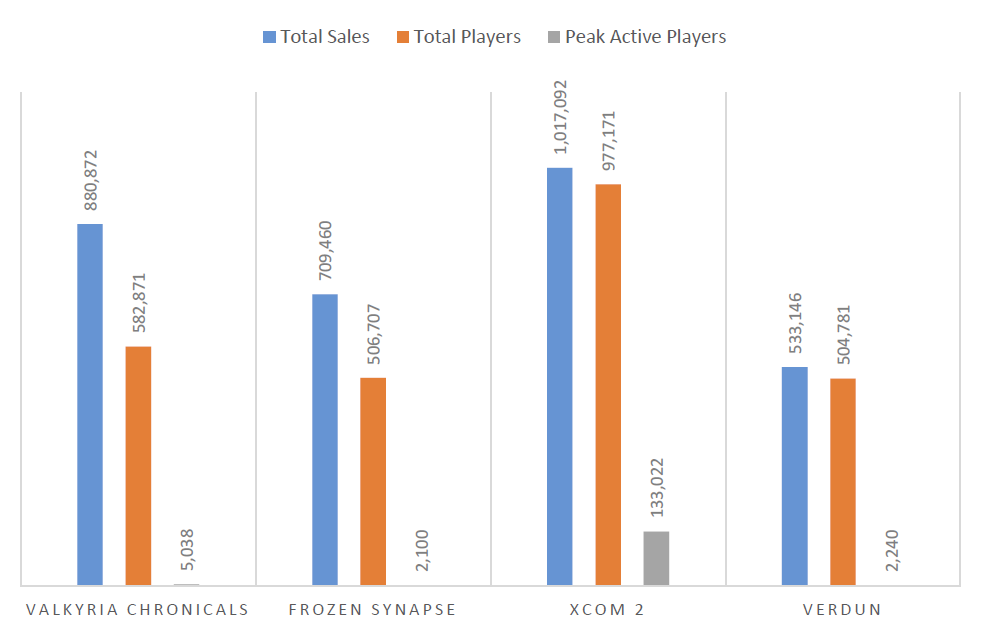
\includegraphics[width=10cm]{SimilarGames}}
\end{frame}




% ////////////////////////// HOW TO EFFECTIVELY MARKET THIS TO THE AUDIENCE 
\begin{frame}{Marketing Strategies}
	\begin{itemize}		
	\item Steam will be the primary distributor for this product.\pause
	\item Have a large social media profile. \pause
	\item Advertise the local multiplayer and easy-to-use network lobby system. \pause
	\item Sell 3D printed items of in-game objects to help raise awareness of the game \pause
	\end{itemize}
\end{frame}

\begin{frame}{Financial Breakdown}
\center{Firelock Financial Breakdown}
	\center{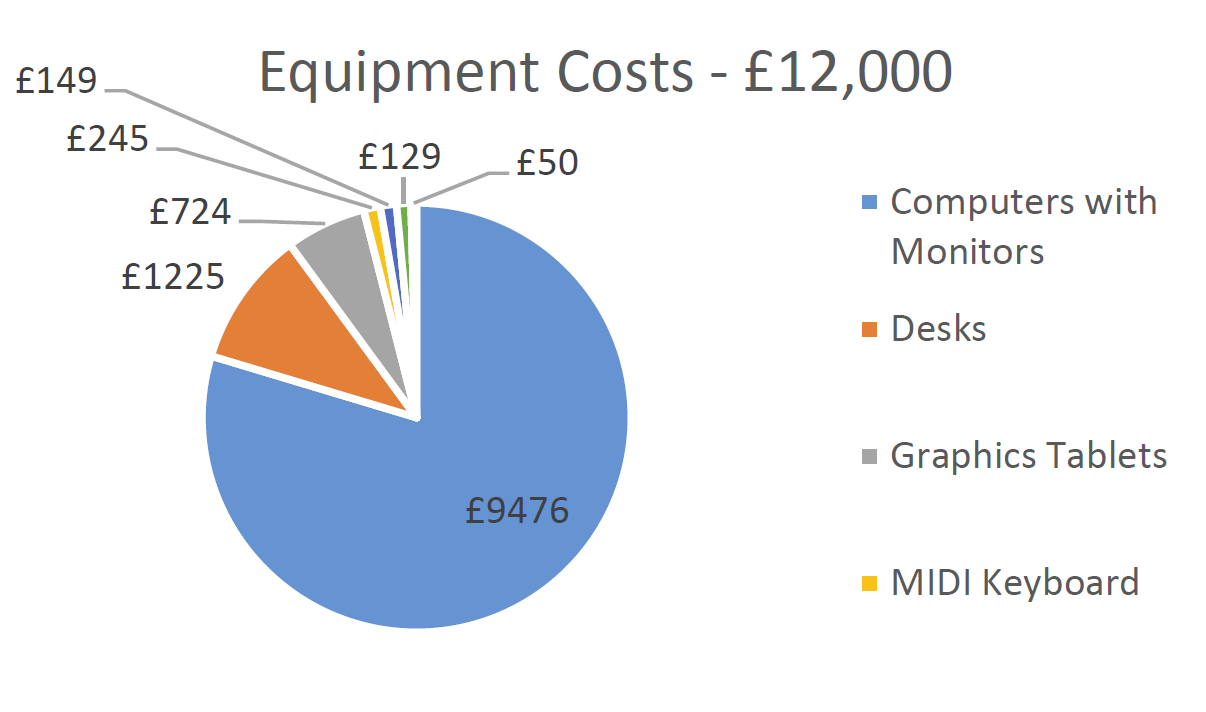
\includegraphics[width=8cm]{Finances}}
\end{frame}

\begin{frame}{Financial Breakdown}
	\center{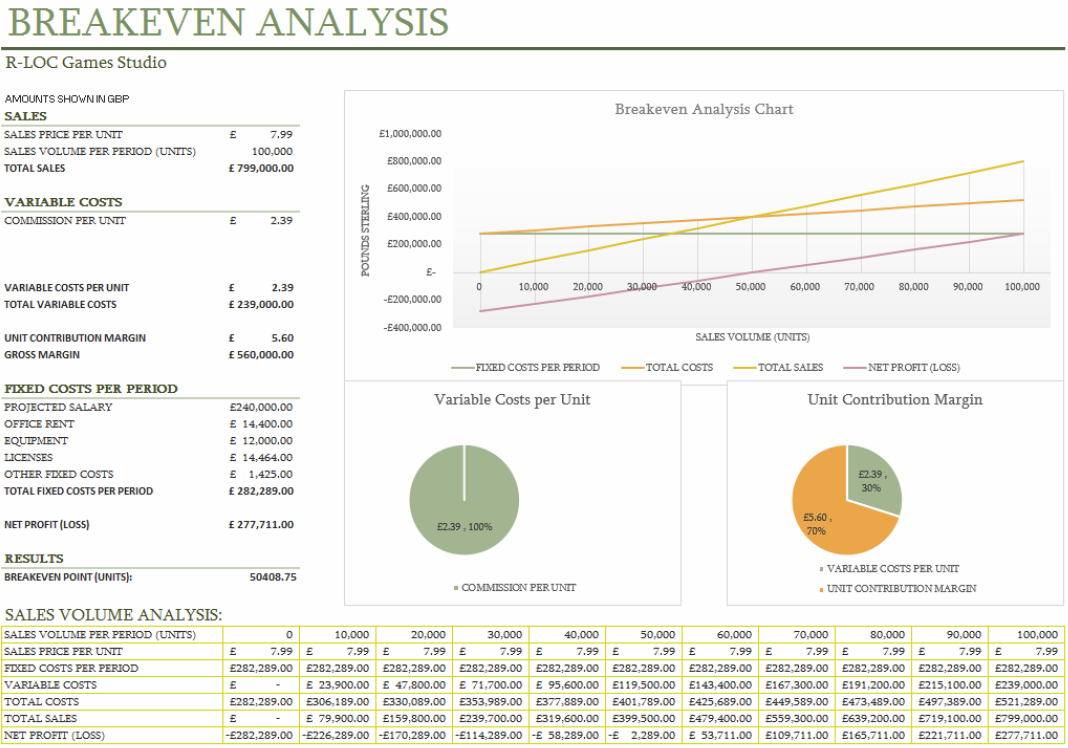
\includegraphics[width=10cm]{Breakeven}}
\end{frame}



\begin{frame}{Thank You}
	\center{Thank You.}
\end{frame}



\end{document}
